%% This is an example first chapter.  You should put chapter/appendix that you
%% write into a separate file, and add a line \include{yourfilename} to
%% main.tex, where `yourfilename.tex' is the name of the chapter/appendix file.
%% You can process specific files by typing their names in at the 
%% \files=
%% prompt when you run the file main.tex through LaTeX.
\chapter{Changing Representations}
The previous chapter described KBRL, a value-iteration
algorithm for solving continuous RL problems.
KBRL uses local averaging to create an approximate value function.
This chapter demonstrates by example how, on some simple MDPs,
local averaging creates
problems---problems that can be fixed by a change in representation.
It then gives a more formal description of the types of MDPs that
cause difficulties.
The chapter concludes with a brief overview of related work from the
representation discovery literature.

\section{Motivating Example}
The discussion section of the background chapter claimed that MDPs with
bumpy value functions are difficult to solve using KBRL.
This section presents a concrete example to show why this is so, and how 
it can be fixed by a change in representation.

Consider the MDP \textit{TWO-ROOM} pictured in Figure 3-1.
\textit{TWO-ROOM} describes an agent in a world with two rooms partially
separated by a thin wall.
The agent is free to move through the open space of the world but cannot
pass through the wall.
A region in one room is marked as the goal.
The agent receives a reward of $-1$ for every time step that it is not in
the goal and a reward of $0$ when it is in the goal.\footnote{Think
of the goal as an absorbing terminal state. Once the agent gets there,
it stays there.}

\begin{figure}[!!!ht]
  \centering
    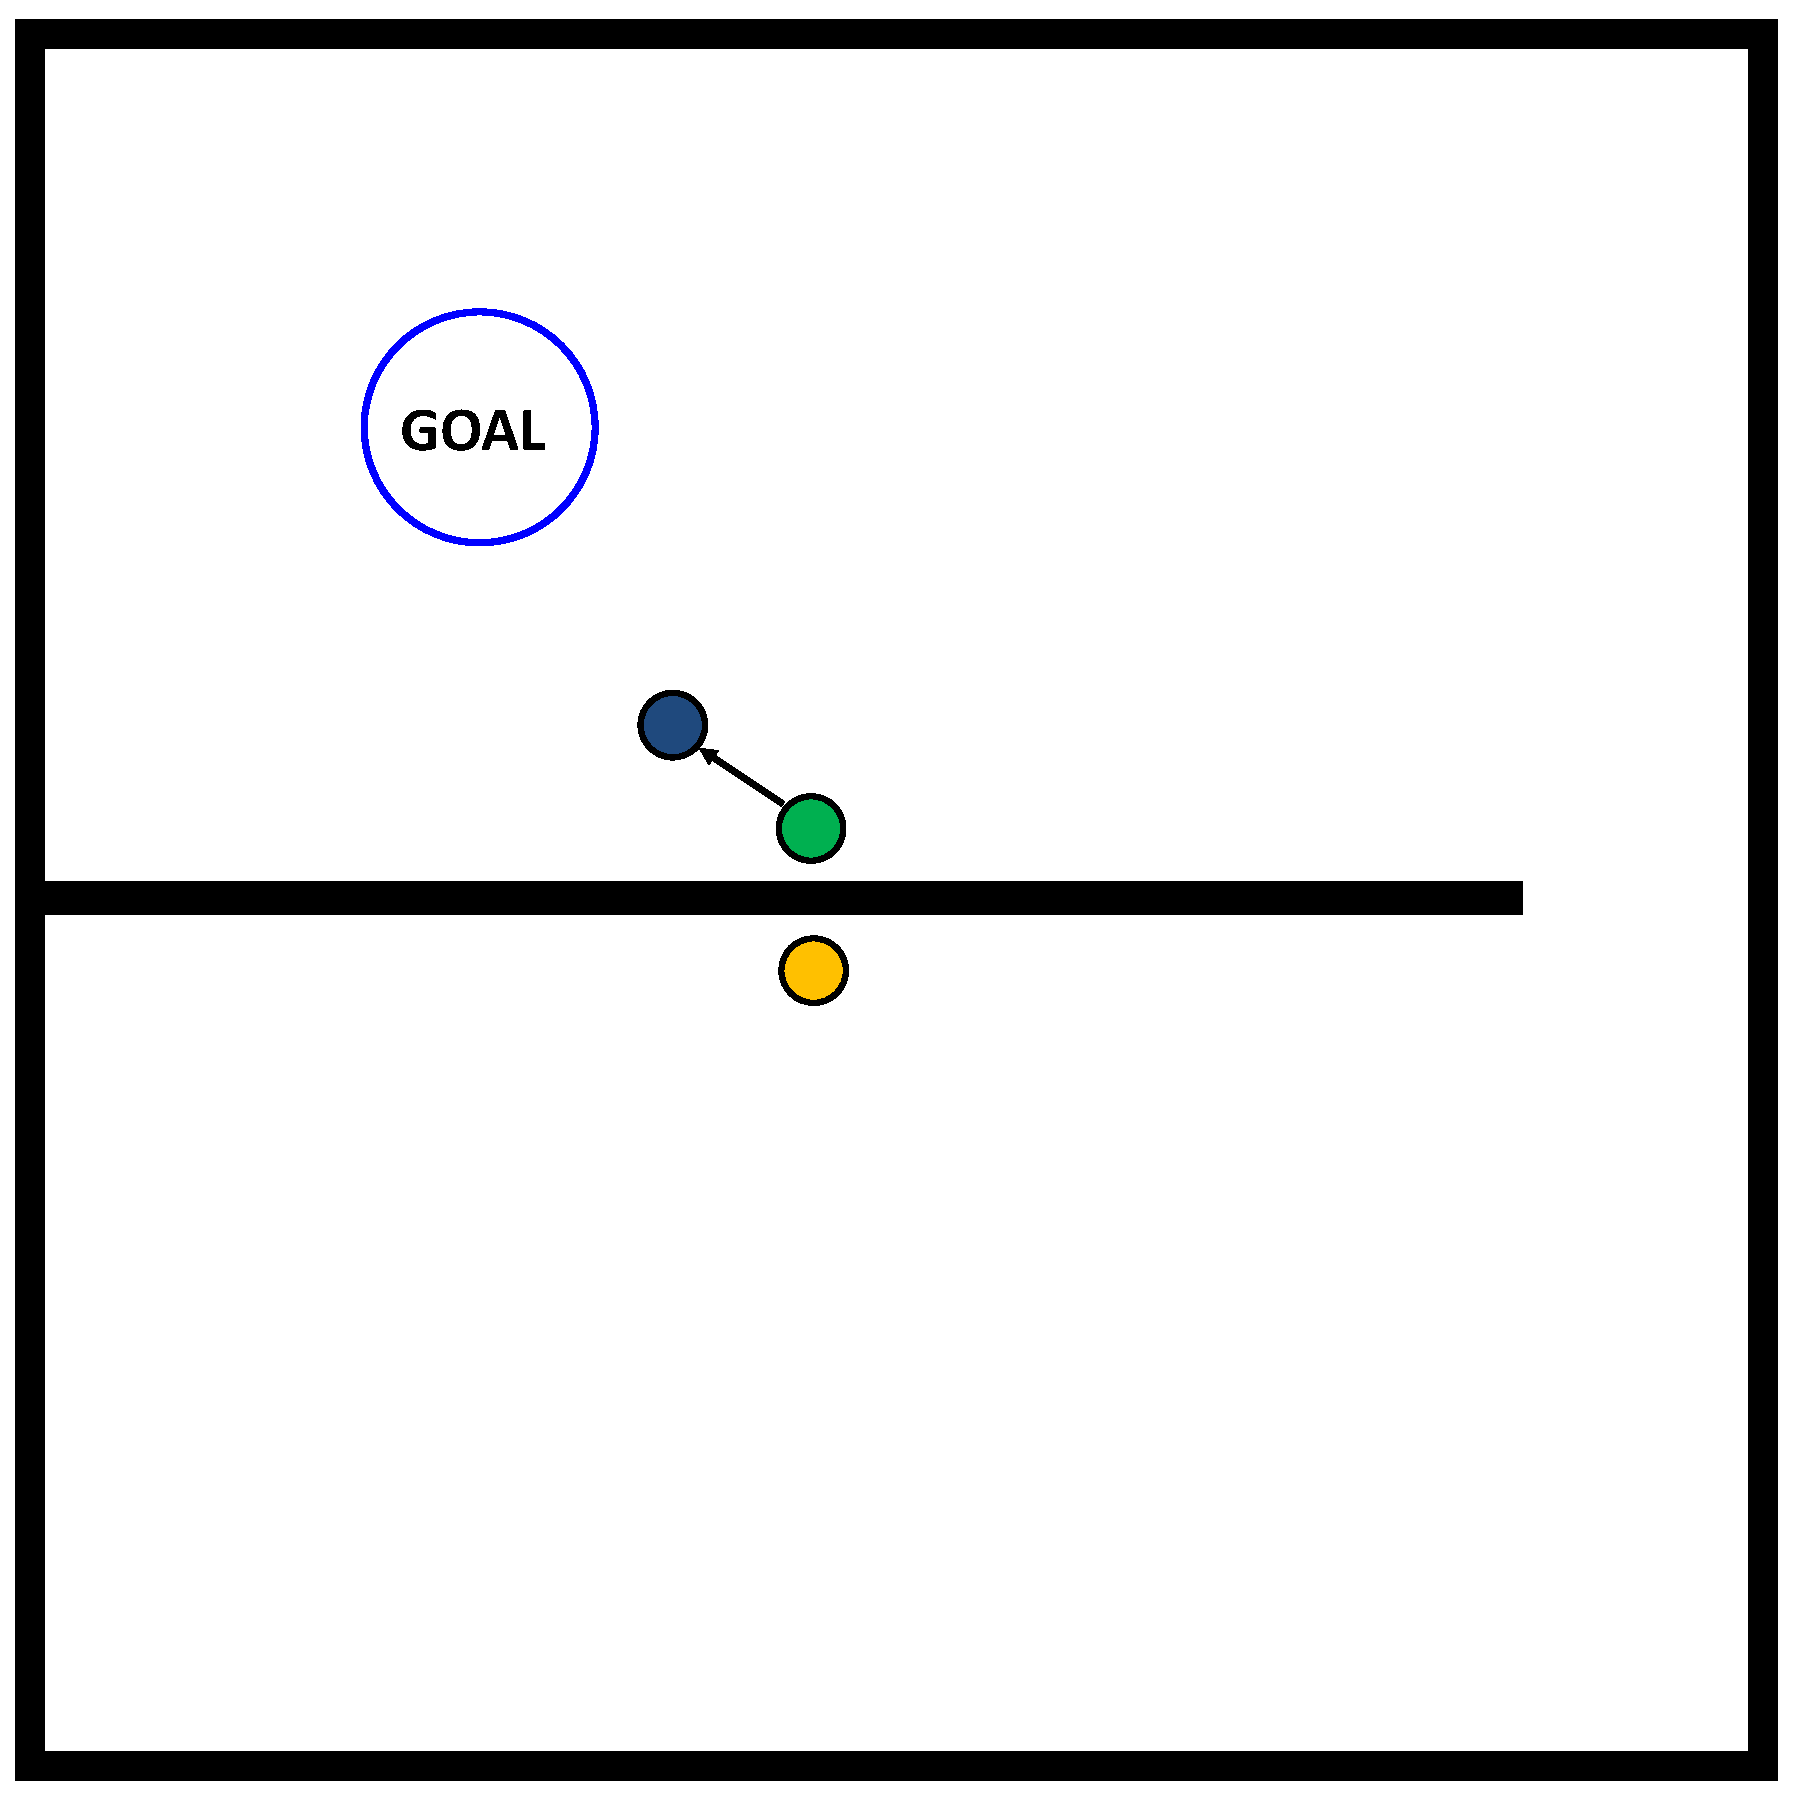
\includegraphics[width=50mm]{figs/tworoom.pdf}
  \caption[The state space of \textit{TWO-ROOM}]
  {The state space of \textit{TWO-ROOM}.
    In this MDP, it would be undesirable to allow a sample transition
    in the top room affect the model of the bottom room.}
\end{figure}

In \textit{TWO-ROOM}, the optimal policy has the agent navigate 
directly to the goal.
Thus, the value of a state is decreasing in the length of the shortest
path from it to the goal.
This means states that are spatially close together, but on opposite sides
of the wall, have significantly different values (see Figure 3-3).
Faithfully representing the steep drop in value across the wall is
necessary for solving \textit{TWO-ROOM}.
To keep KBRL from smoothing out the value cliff, one would need to use
a small bandwidth.
Compensating for the variance that comes from working with
small bandwidths requires using a large set of sample transitions.
This makes the domain much harder for KBRL than it ought to be.

\begin{figure}[!!!ht]
  \centering
    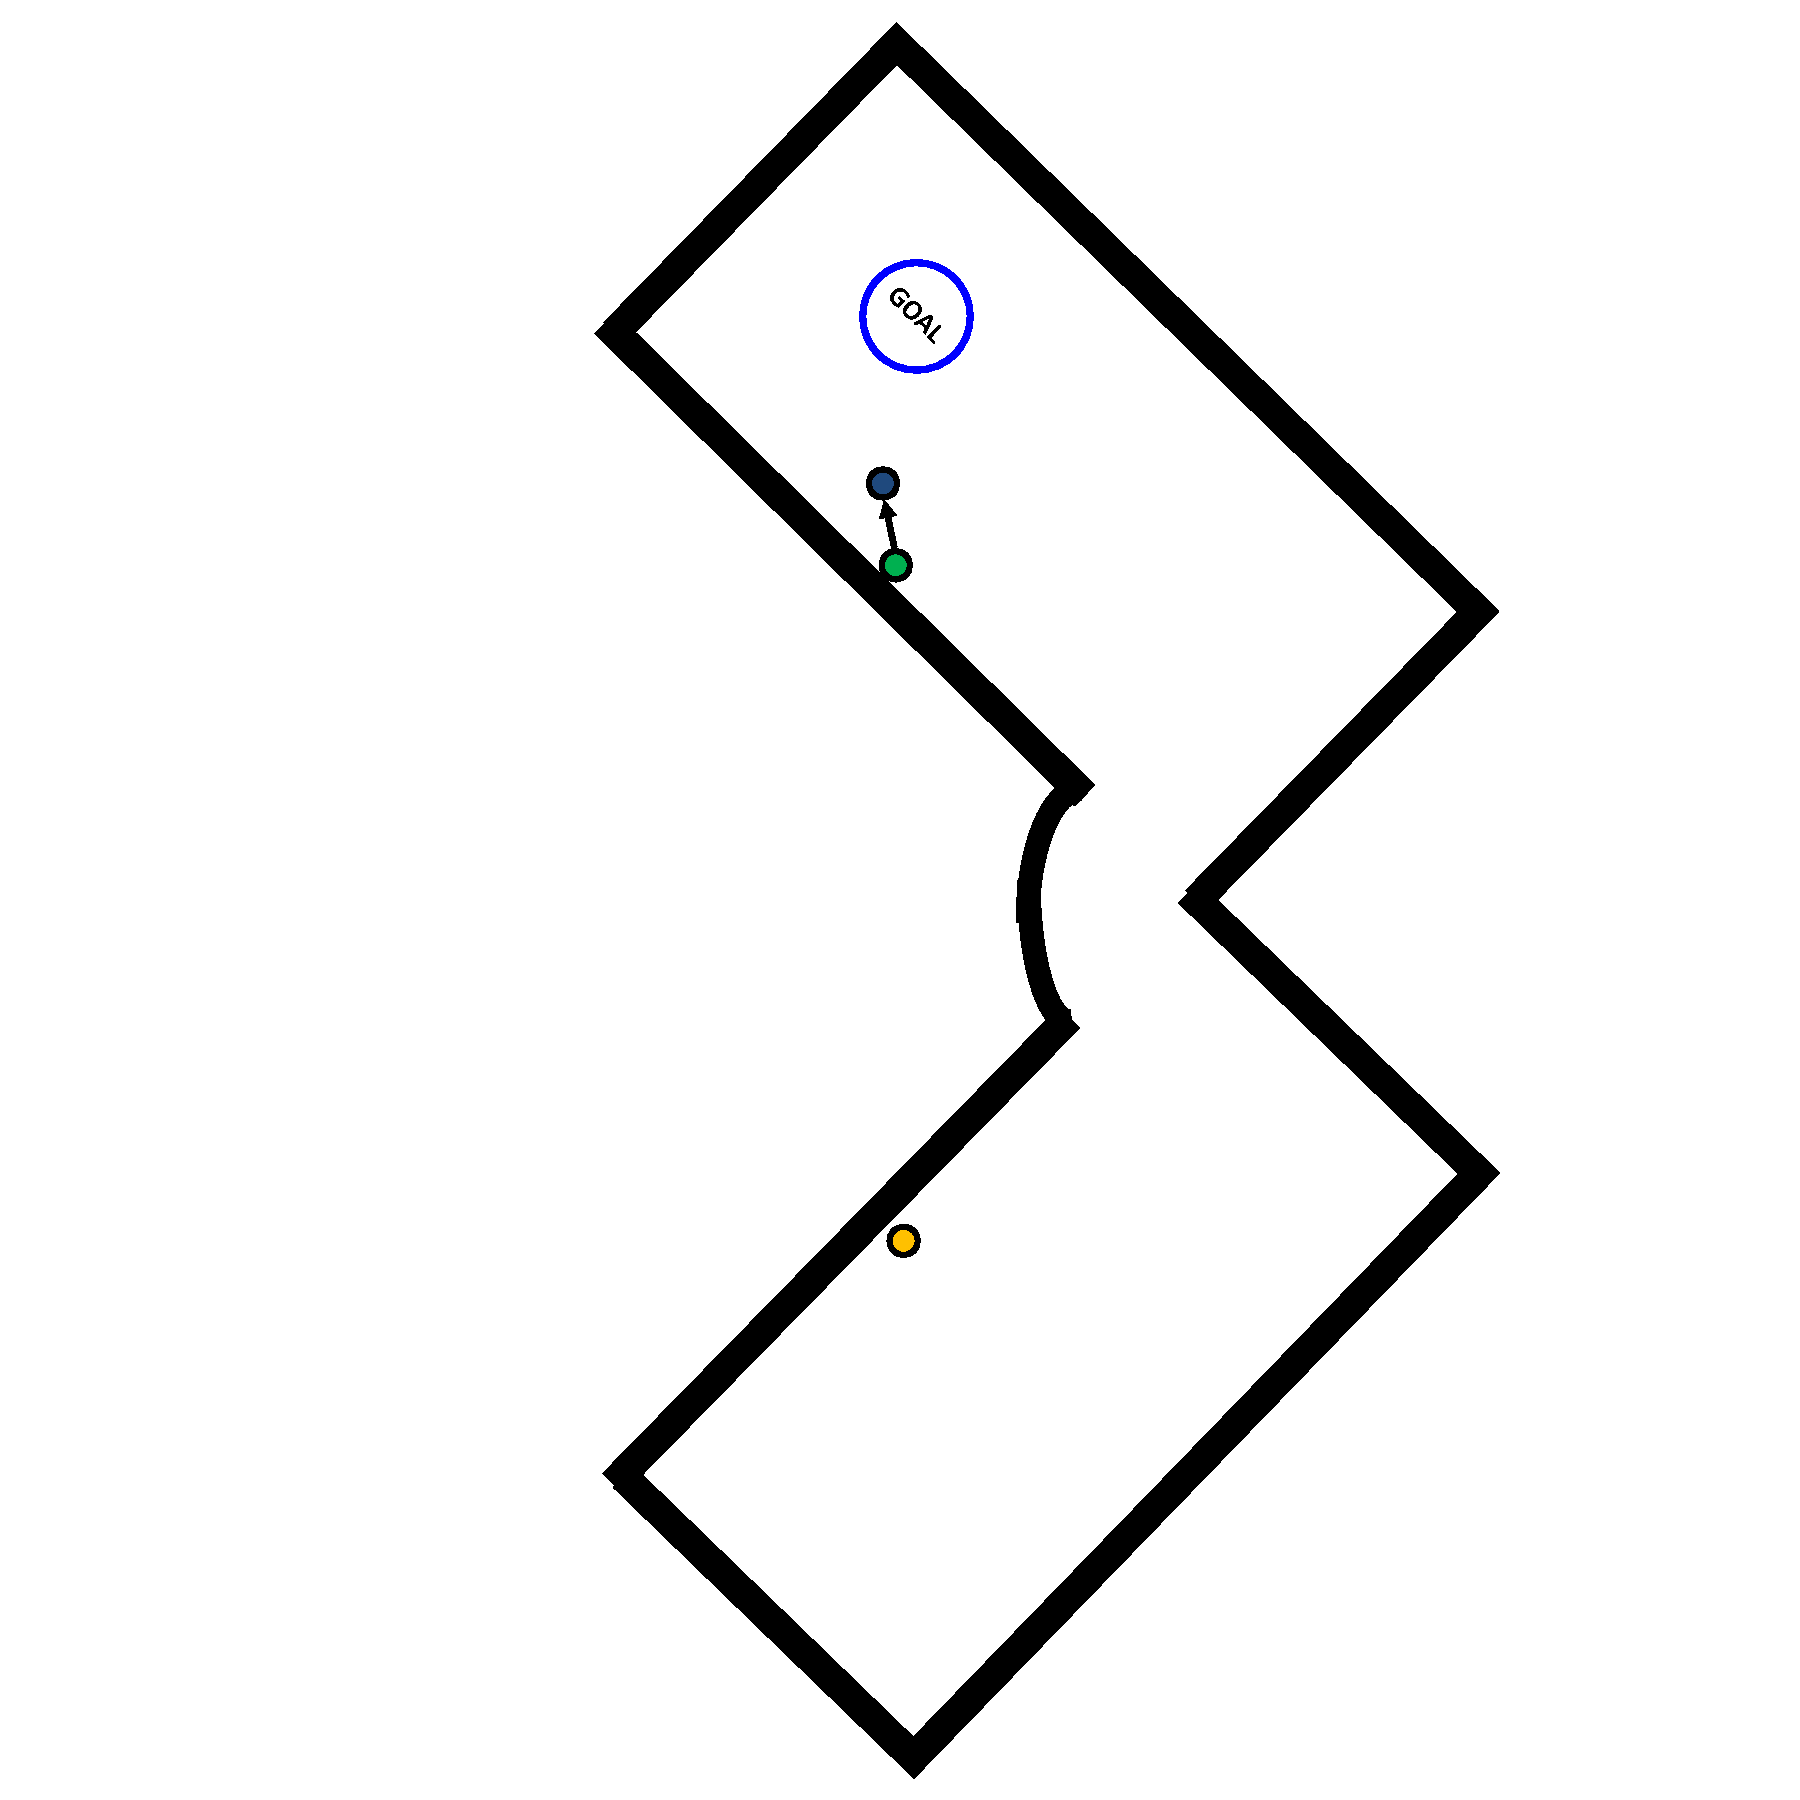
\includegraphics[width=90mm]{figs/tf2room.pdf}
  \caption[Alternative representation for the state space of
      \textit{TWO-ROOM}]
      {An alternative representation for the state space of
\textit{TWO-ROOM}. In this representation there is little risk of
averaging across the wall.}
  \label{fig:tf2rm}
\end{figure}

Now consider a representation for the state space where the wall is
``opened up'' so that states on opposite sides of it are no longer close
(Figure 3-2).
In this representation, the distance between two points says something
about their similarity.
This makes local averaging safe to do with a much larger bandwidth and
far fewer points.

\begin{figure}[!!!ht]
  \centering
    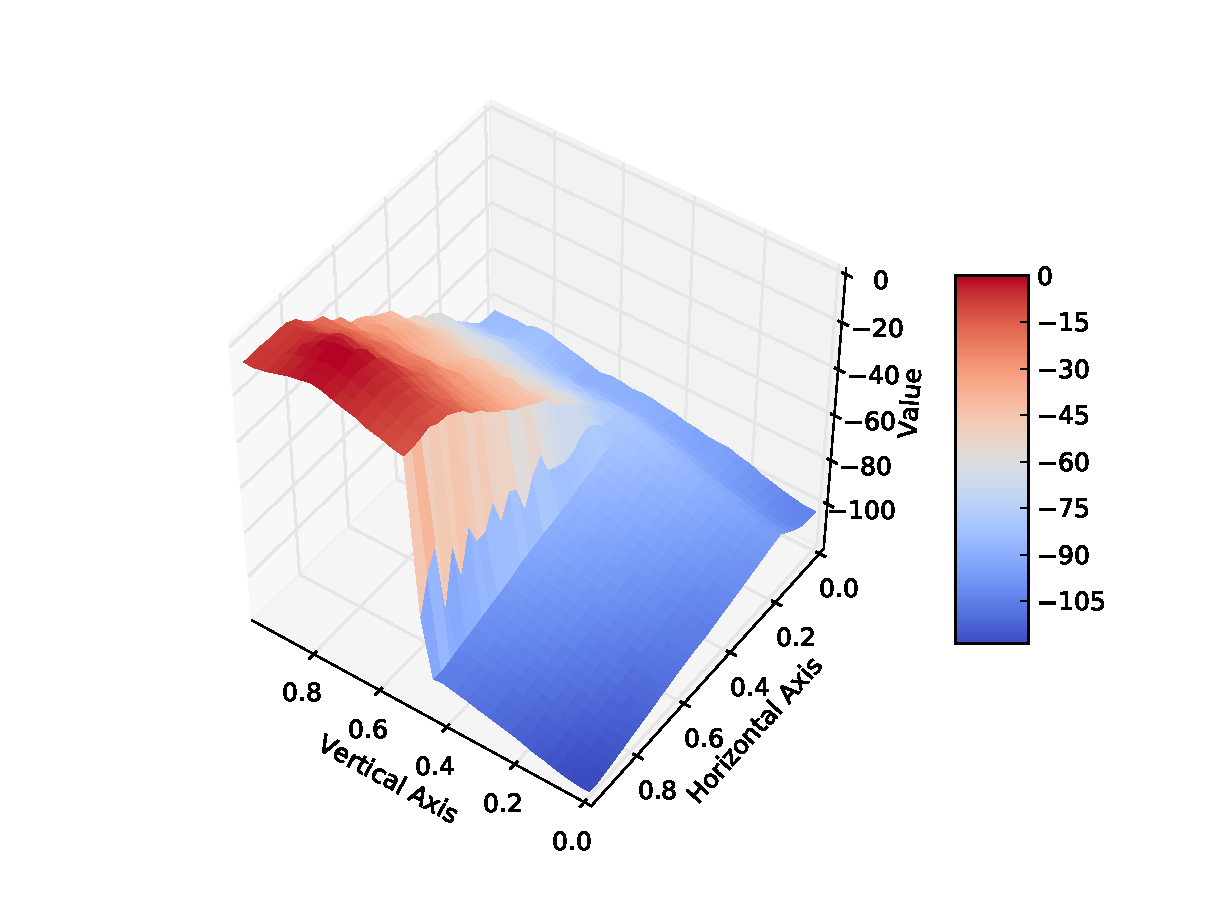
\includegraphics[width=110mm]{figs/true2rmvf.pdf}
  \caption[\textit{TWO-ROOM} value function learned using small bandwidth]
  {The value function of \textit{TWO-ROOM} as approximated by
  KBRL in the original space with a bandwidth of $.01$. It captures the
  discontinuity adequately. Notice the ripples in the top room. These are
  artifacts of the small bandwidth.}
  \label{fig:og2rm}
\end{figure}

\begin{figure}[!!!ht]
  \centering
    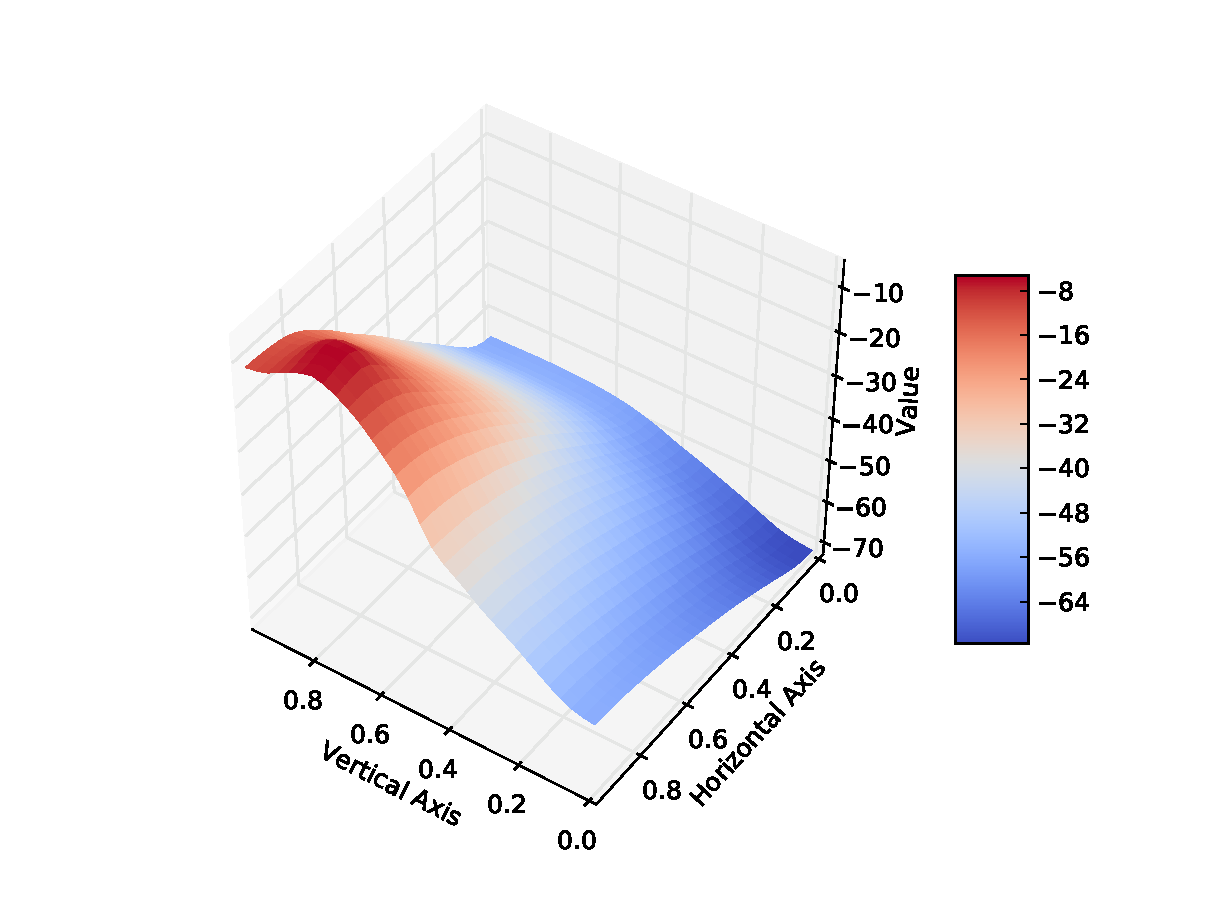
\includegraphics[width=110mm]{figs/blur2rmvf.pdf}
  \caption[\textit{TWO-ROOM} value function learned using large bandwidth]
  {The value function of \textit{TWO-ROOM} as approximated by
  KBRL in the original space, this time with a bandwidth of $.06$.
  Note how poorly it models the wall.
  The policy that results from this value function
  has the agent attempt to walk through the wall.}
  \label{fig:bl2rm}
\end{figure}

\begin{figure}[!!!ht]
  \centering
    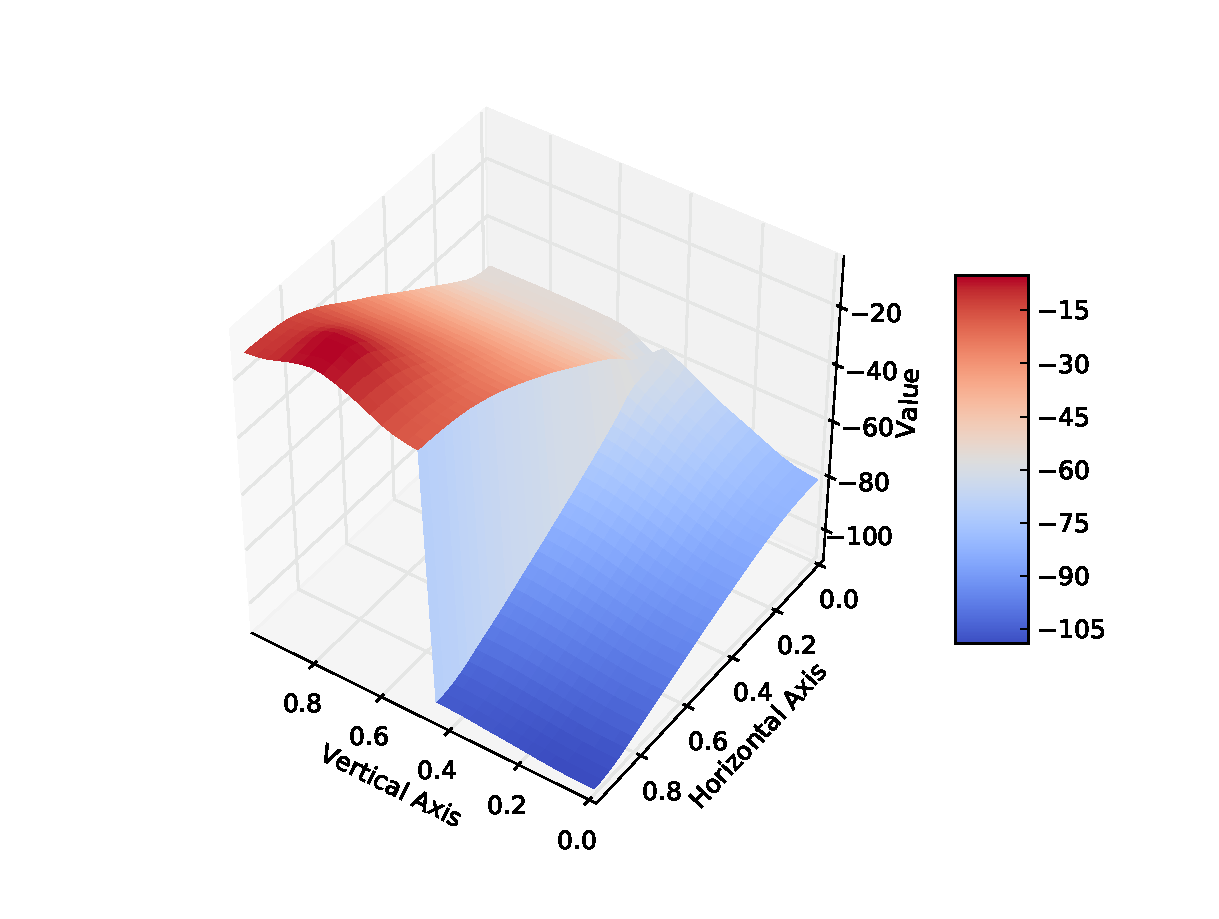
\includegraphics[width=110mm]{figs/tf2rmvf.pdf}
  \caption[\textit{TWO-ROOM} value function learned in the transformed space]
  {The value function of \textit{TWO-ROOM} approximated by
  KBRL in the transformed space and mapped back to the original toplology
  (bandwidth of $.06$).
  This captures the discontinuity well and has no ripples.
  All three plots (3-3, 3-4, 3-5) above were created using the same
set of sample transitions.}
  \label{fig:tfv2rm}
\end{figure}

\section{Discussion}
By any reasonable measure, \textit{TWO-ROOM} is a simple domain,
yet it poses a challenge for KBRL simply because its value function
has a discontinuity.
KBRL is intended for problems with smooth value functions, so
it is understandable that it would do poorly in this domain.
The failure is not one of technique, but of representation.
The original representation of the MDP is not well suited for
representing the value function.
After a simple transformation, the domain becomes easy for KBRL.

The discontinuity in \textit{TWO-ROOM}'s value function comes from
the local connectivity of the state space;
this is not the only way discontinuities arise.
Discontinuities can also come from non-local properties of the MDP.
Consider the following minor modification to \textit{TWO-ROOM}:
the agent can run through the wall if it hits it with enough momentum,
but building up the necessary momentum requires the agent to accelerate
through some distance, $\delta$.
In this formulation, states where the agent is on pace to break though the wall
have a very different value from the ones where it isn't.
Note that these states may be arbitrarily close to each other and up to
a distance of $\delta$ from the wall.\footnote{To see another discontinuity
of this form, see MountainCar in the Results chapter.}
There is no local information that can help differentiate these states.

Transition dynamics are not the only possible cause of roughness in
the value function.
Value cliffs can also result from the underlying reward structure of the MDP.
An example of this is \textit{TWO-ROOM} where the wall is not a physical
barrier but a region of low reward.
With this modification, there is nothing about the topology of the space that
would suggest a discontinuity but the value function is as if there is a wall.

Many of the benchmark problems in the reinforcement learning literature are
like \textit{TWO-ROOM};
their value functions are smooth but for a handful of discontinuities.
This suggests that they too could benefit from a change in representation.
In \textit{TWO-ROOM} we were able to use domain knowledge to engineer a new
representation. This is not always possible or desirable.
Ideally, the agent would discover a good representation in the process
of solving the problem.

\section{The Best Representation}
The previous sections provide a high level discussion of the advantage of
changing representations.
The existence of regions of the state space where the value function
changes rapidly is problematic for KBRL.
Our solution is to transform the state space in a way that smooths out the
value function.
We now make these ideas concrete and attempt to gain insight about the
best possible transform.

Let $f:X \to Y$ be a non-constant, Lipschitz-continuous\footnote{
Lipschitz-continuity roughly corresponds to having a bounded slope.
A function, $f$ is Lipschitz-continuous if there exists a $K$ such that
for all $x$, $x'$ in the domain of $f$,
$K \geq \frac{|f(x) - f(x')|}{\|x - x'\|}$.
A $K$ satisfying this equation is called a Lipschitz constant for $f$.},
and bounded function with compact, connected support.
Denote the diameter of the support as $diam(X) = \max_{x,x' \in X}||x - x'||$
and let $f_{max}$ and $f_{min}$ denote the maximum and minimum values 
respectively of $f$ on $X$.
Let $K_f$ denote the smallest Lipschitz constant for $f$.

\begin{definition}
The \textbf{wrinkliness} of $f$ is
$w(f) = K_f \cdot \frac{diam(X)}{f_{max} - f_{min}}$.
\end{definition}

Consider the function $g(x) = \mathrm{log}(x^2-7x+20)$ with domain $[1,100]$.
The extrema of $g$ are $g_{min} \approx 2.05$ and that $g_{max} \approx 9.14$.
The maximum slope of $g$ is $\approx .36$.
From this we can calculate that $w(g)\approx.36*(100-1)/(9.14-2.05) = 5.01$.

The wrinkliness of a function is the ratio of its maximum slope to the
minimum slope it would need to pass through the extrema on its domain.
Wrinkliness is a measure of how non-linear a function is.
Note that $w(f) \geq 1$. Call $f$ \textbf{wrinkle-free} if $w(f) = 1$. 
The only way $f$ can be wrinkle free is if it attains its global extrema
at points separated by the diameter and its slope never exceeds
$\frac{f_{max} - f_{min}}{diam(X)}$.

\begin{definition}
The \textbf{inverse target slope} of $f$ is
$\mu_f = \frac{diam(X)}{f_{max} - f_{min}}$.
\end{definition}

An example of a wrinkle-free function is $f(x) = c x + d$ for some
constants $c$ and $d$. All wrinkle-free functions in one-dimension are of
this form. In higher dimensions, wrinkle-free functions can be more
complicated.

Now consider a transform $\Phi: X \to X'$ ($X'$ compact and connected)
satisfying $f(x_1) \neq f(x_2) \implies \Phi(x_1) \neq \Phi(x_2)$.
Let $f_\Phi : X' \to Y$ be the function satisfying $f_\Phi(\Phi(x)) = f(x)$.
The existence of $f_\Phi$ follows from the constraint that $\Phi$ not map
points with the different values to the same point.
If $f_\Phi$ is Lipschitz-continuous, we can define wrinkle-ironing transforms
as follows:

\begin{definition}
$\Phi$ is a \textbf{wrinkle-ironing transform (WIT)} if $w(f_\Phi) \leq w(f)$.
\end{definition}

Consider the transform $\Phi_{\log}(x) = \log(x)$.
Applying $\Phi_{\log}$ to the domain of $g$ above gives the new domain
$[0,\log(100)]$.
The $g_\Phi$ satisfying $g_\Phi(\Phi_{\log}(x)) = g(x)$ is
$G(x) = \log(e^{2x}-7e^x+20)$. It has the same extrema as $g$ and a
maximum slope of $2.61$.
From this we can calculate that
$w(G)\approx2.61*\mathrm{log}(100)/(9.14-2.05)=1.69$.
This means $\Phi_{log}$ is a wrinkle ironing transform for $g$.

\begin{figure}[!htb]
  \minipage{0.5\textwidth}
    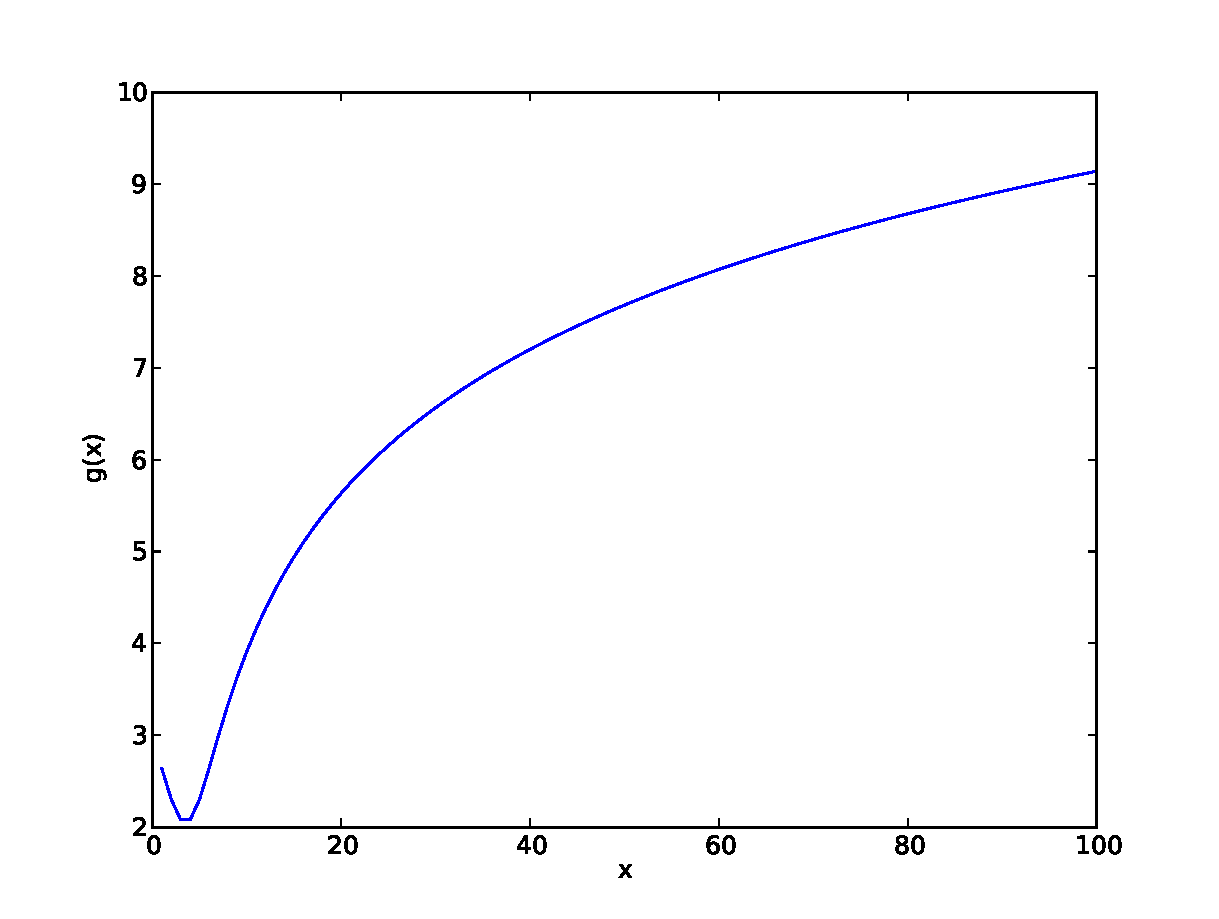
\includegraphics[width=\linewidth]{figs/gp1.pdf}
  \endminipage\hfill
  \minipage{0.5\textwidth}
    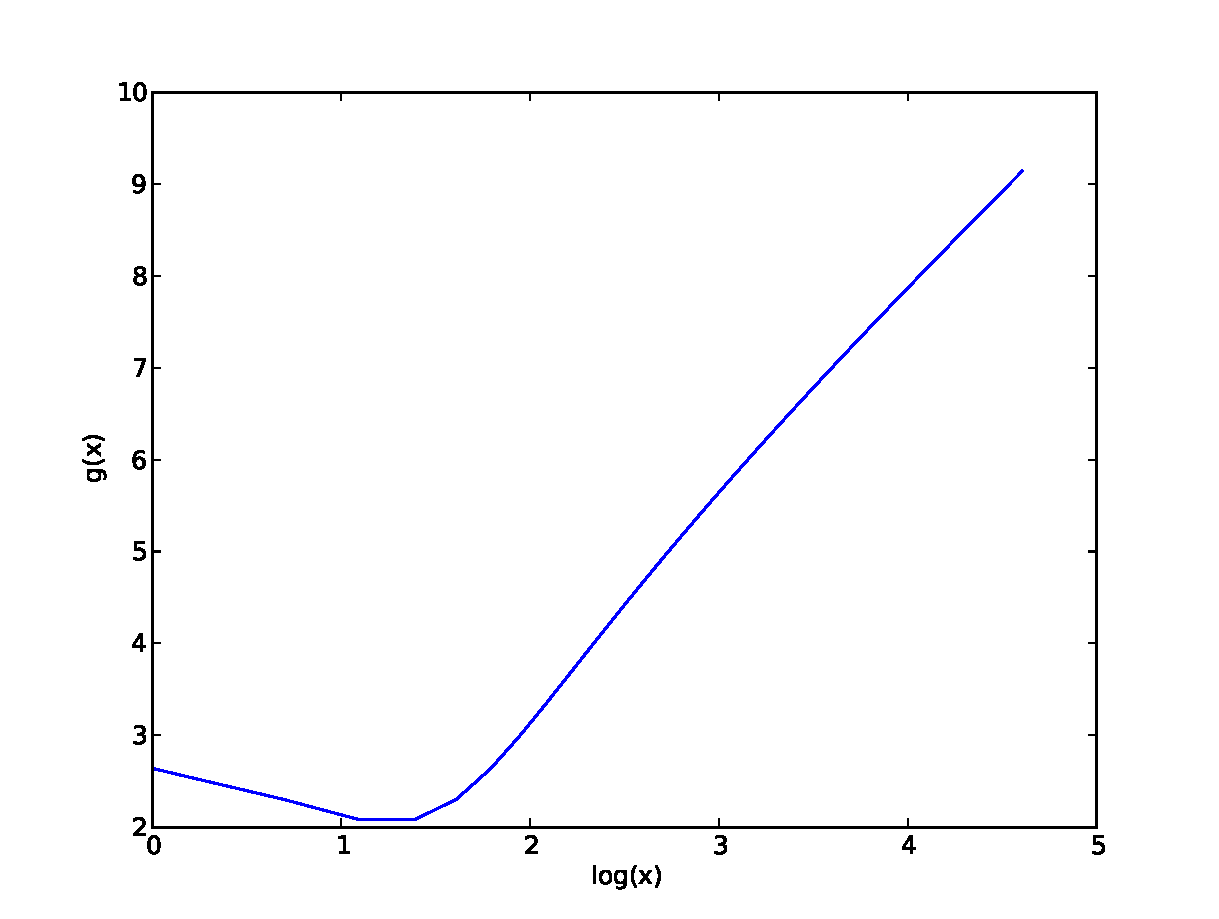
\includegraphics[width=\linewidth]{figs/gp2.pdf}
  \endminipage
\caption[Wrinkle-Ironing Transform Example]{On the left, $g(x)$ plotted on its
  original domain. On the right, $g(x)$ plotted against $\log(x)$.
  Note how the WIT straightened out the function.}
\end{figure}

Local-averaging kernel-smoothers work by assuming the function being
approximated is locally flat.
As a result, the only function they can represent without error is
the constant function, $f(x) = c$ for some $c$.
In the special case where the domain is unbounded and the sample points uniformly
cover the domain, kernel-smoothers can also represent lines without error.
\footnote{When the domain is bounded the kernel-smoother produces an
approximation that is biased at the boundaries.
The implications of this are discussed in detail in the next chapter.}
This means one can use wrinkliness as a measure of how poorly a
kernel smoother will represent a function.

KBRL approximates the Q-Values of an MDP using kernel smoothers of the form
$k(\frac{||s - x||}{b})$.
If we assume that wrinkliness is a reasonable measure of fit quality,
it follows that without lowering the bandwidth, one can get a higher
fidelity approximation by applying a wrinkle-ironing transform,
$\Phi$, to the state space and working with
$k(\frac{||\Phi(s) - \Phi(x)||}{b})$.
Since it may be the case that no single transform can iron the wrinkles
in all the Q-Values, one should use a separate transform $\Phi^a$ for
each action, $a$.

Note that applying a transform that stretches the state space uniformly in
all directions is equivalent to shrinking the bandwidth.
We exclude will such transforms by adding the constraint that the
transforms not increase the diameter of the state space.

All this leads us to the conclusion that the best possible transform
is the wrinkle-free $\Phi^{a^*}(s) = \mu_{Q^a} \cdot Q(s,a)$, we define
this to be \textbf{the Platonic Transform}.
This is a disheartening result;
it suggests one needs to know the Q-Values to produce a transform that makes
it easy to approximate the Q-Values.
The next chapter introduces an algorithm that attempts to bootstrap a
solution to this problem, iteratively approximating the Q-Values then the
transform.

A possible concern is that transforming the state space in this way may alter
the optimal policy.
The transform $\Phi^*$ described above is a $Q^*$-irrelevance abstraction
\cite{lietal} since
$\Phi^*(s_1) = \Phi^*(s_2) \implies Q(s_1, a) = Q(s_2, a)$ for all $a$.
Q-learning with a $Q^*$-irrelevance
abstraction converges to the optimal state-action value function in the
underlying MDP. 
This means using $\Phi^*$ in KBRL will not lower the solution quality.

\section{Related Work}
Representation discovery is not a novel concept.
The past decade has seen several representation discovery algorithms
in a number of different settings.
The following are the ones most closely related to this thesis,
presented in chronological order.

\begin{description}
\item[ST-Isomap]
\cite{jenkins} is an extension of Isomap \cite{tenen} that takes temporal
information into account.
It uses a modified nearest neighbours algorithm to construct a graph from
the dataset.
It then unfolds the graph using MDS \cite{mds} on the matrix of shortest-path
distances.

\item[Action-Respecting Embedding] \cite{bowling} constructs a graph from
the set of sample transitions using nearest neighbours with the
neighbourhood sizes determined by the effect of an action.
It then unrolls and morphs the graph using a semidefinite program whose
constraints ensure that neighbourhoods are preserved and that each action
corresponds to a rotation-plus-translation.

\item[BEBF] \cite{parr} is an algorithm for discovering a set of basis
functions for use in a linear approximation architecture. It iteratively
adds new bases using the approximation error from the old bases.

\item[PVFs] \cite{pvf} constructs a graph embedding using nearest
neighbours on the dataset then attempts to represent the value function
in terms of the eigenfunctions of the graph Laplacian.
PVFs can be computationally intensive to create, but recent work on
Incremental SFAs \cite{incsfa} has made it more tractable.

\item[Predictive Projections] \cite{sprague} finds a linear transformation
that projects the original space into a space where state values are more
highly correlated.
\end{description}

These algorithms all had considerable success in dealing with the problems
they were designed to address, but they are not versatile enough to
generalize to other types of problems. For instance, they all fail on some
version of \textit{TWO-ROOM} presented above.

The algorithms that build a graph representation (ST-Isomap, PVFs, and ARE)
can only create representations that fix discontinuities that come from the
local topology of the state space.
They cannot deal with the case where the agent can run through the wall or
where the wall is replaced by a region of low reward.
It is not possible to build a representation that is universally useful
without considering the reward function.
ST-Isomap and PVFs are further limited by the fact that the abstractions they
produce are neighbourhood preserving---they do not stretch or squash the
domain.
One can imagine cases where the best transform involves distorting the state
space.
Consider, for instance, \textit{TWO-ROOM} modified so that the vertical axis
is measured in meters and the horizontal axis is measured in miles.
A good transform would stretch the axes so that the units matched.

Predictive Projection is severely limited by the fact that it only finds linear
transformations. Few problems of interest can be represented well after a
linear transformation. Predictive Projection cannot make a better
representation for any version of \textit{TWO-ROOM}.

BEBF does not learn a representation of the state space, instead it
learns a basis for representing the value function.
BEBF is similar in spirit to what we are trying to accomplish:
it involves iteratively approximating the value function then updating the
representation; however, since BEBF is parametric, the bases
it considers are tied to the native representation of the problem.

None of the algorithms above have been applied in a non-parametric
reinforcement learning setting. 
This makes it difficult to compare them to the work presented in this thesis.
To the best of my knowledge, there is no literature on non-parametric
representation learning.
Thus, results in this thesis are only compared against the results of
KBRL and KBSF.

Now that the problem of representation discovery has been sufficiently
motivated, we can proceed to describing an algorithm for it.
